\tikzstyle{input_neuron}=[circle,draw=red!50,fill=red!10,thick,minimum size=6mm]
\tikzstyle{hidden_neuron}=[circle,draw=blue!50,fill=cyan!10,thick,minimum size=6mm]
\tikzstyle{output_neuron}=[circle,draw=green!50,fill=green!20,thick,minimum size=6mm]
\tikzstyle{input}=[circle,draw=black!50,fill=black!20,thick,minimum size=6mm]

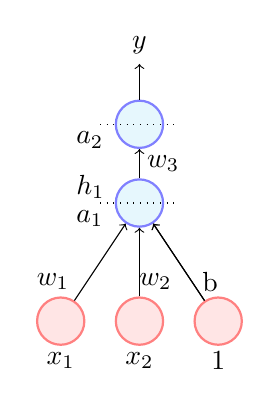
\begin{tikzpicture}

	\node (input1) at (1,2)  {$x_{1}$};
	\node (input2) at (2,2)  {$x_{2}$};
	\node (input3) at (3,2)  {$1$};
	\node (output) at (2,6)  {$y$};
	
	\node [hidden_neuron] (hidden_neuron2) at (2,5) {};
	\node [hidden_neuron] (hidden_neuron1) at (2,4)  {} ;
	\node [input_neuron] (input_neuron1) at (1,2.5) {};
	\node [input_neuron] (input_neuron2) at (2,2.5) {};
	\node [input_neuron] (input_neuron3) at (3,2.5) {};
	\draw [->] (input_neuron1) -- (hidden_neuron1);
	\draw [->] (input_neuron2) -- (hidden_neuron1);
	\draw [->] (input_neuron3) -- (hidden_neuron1);
	\draw [->] (input_neuron3) -- (hidden_neuron1);
	\draw [->] (hidden_neuron1) -- (hidden_neuron2);
	\draw [->] (hidden_neuron2) -- (output);
	
	\draw [dotted] (1.5,5) -- (2.5,5);
	\draw [dotted] (1.5,4) -- (2.5,4);
	\node[text width=0.005cm] at (0.7,3) {$w_1$};
	\node[text width=0.005cm] at (2,3) {$w_2$};
	\node[text width=0.005cm] at (2.8,3) {b};
	\node[text width=0.005cm] at (1.2,4.2) {$h_1$};
	\node[text width=0.005cm] at (1.2,3.8) {$a_1$};
	%\node[text width=0.005cm] at (1.2,5.2) {$h_2$};
	\node[text width=0.005cm] at (1.2,4.8) {$a_2$};
	
	\node[text width=0.005cm] at (2.1,4.5) {$w_3$};
	
\end{tikzpicture}